\subsubsection{Reset GBTx ASIC}
Sometimes GBTx ASIC will not be properly reset by reprogramming, or it may have
erratic/unexpected behaviors.
In such case, a manual jumper reset can be performed on the GBTx DB to reset
GBTx ASIC.
Follow the \autoref{fig:gbtx-reset} to reset GBTx ASIC.

\begin{figure}[!ht]
\centering
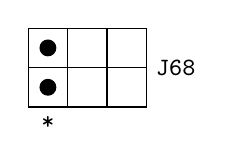
\begin{tikzpicture}
    % Pins
    \draw (0,0) rectangle (1.5,-1);
    \draw (0,-0.5) to (1.5,-0.5);
    \draw (0.5,0) to (0.5,-1);
    \draw (1,0) to (1,-1);

    % PCB labels
    \coordinate (A) at (1.5,-0.5);
    \node at (A) [right] {\small\texttt{J68}};
    \coordinate (B) at (0.25,-1);
    \node at (B) [below] {\small\texttt{*}};

    % Pins that need to be connected
    \draw [black,fill] (0.25,-0.75) circle [radius=0.1];
    \draw [black,fill] (0.25,-0.25) circle [radius=0.1];
\end{tikzpicture}
\caption{
    Schematic for resetting GBTx ASIC. A jumper should be used to connect the
    two pins marked above.
}
\label{fig:gbtx-reset}
\end{figure}
